% =============================================================================
% COMPSCI-603 Group Project --- Deliverable 4: Final Report
% Team: Chengtao Lin, Yongye Tan, Nalongsone Danddank
% Compile with: pdflatex d4_results.tex
% =============================================================================
\documentclass[letterpaper, 10 pt, conference]{ieeeconf/ieeeconf}

\IEEEoverridecommandlockouts
\overrideIEEEmargins

\usepackage{amsmath,amssymb}
\usepackage{graphicx}
\usepackage{booktabs}
\usepackage{array}
\usepackage{url}
\usepackage{hyperref}
\usepackage{tikz}
\usetikzlibrary{shapes.geometric, arrows.meta, positioning, fit, backgrounds}

\begin{document}

\title{\LARGE \bf
Autonomous Symbol Search on a Physical Mobile Robot:\\
Design, Adaptation, and Real-World Deployment
}

\author{Chengtao Lin, Yongye Tan, and Nalongsone Danddank\\
University of Massachusetts Amherst\\
\texttt{chengtaolin@umass.edu},
\texttt{yongyetan@umass.edu},
\texttt{ndanddank@umass.edu}}

\maketitle
\thispagestyle{empty}
\pagestyle{empty}

% -----------------------------------------------------------------------------
\begin{abstract}
This paper presents our COMPSCI-603 final group project: designing, implementing,
and deploying an autonomous symbol-search system on the physical Triton mobile
robot.
The original goal was a complete RGB-D pipeline in which the robot would explore
an environment using a Q-learning policy, detect requested printed symbols
(circle, square, triangle, star), localize each symbol in 3-D using the Intel
RealSense D435 depth stream, store detections in a persistent JSON symbol map,
and navigate to the requested symbol.
We implemented all major subsystems: a Gazebo Q-learning trainer, a classical
OpenCV symbol detector, a depth-backprojection localizer, a persistent symbol
map, a navigation controller, and a neural-network recognition prototype.
During physical deployment, two important limitations arose.
First, the Q-learning policy trained in Gazebo did not transfer reliably to
the real kitchen, producing oscillatory behavior instead of smooth exploration;
we replaced it with a LiDAR-based reactive explorer.
Second, the RealSense D435 camera on the robot enumerated as USB~2.0 (480~Mbps)
rather than USB~3.0 (5000~Mbps), making the aligned RGB-D stream unstable and
forcing us to redesign the final demo as a color-only pipeline.
We also moved the final demo environment from the kitchen to an open indoor
room, which provided better visibility for the printed symbols.

The final real-robot demo used LiDAR reactive exploration, low-bandwidth
OpenCV 2-D triangle detection, and a debounced stop-on-detection monitor.
The monitor required at least three high-confidence triangle detections
(confidence $\geq 0.80$) within a 2-second window before stopping the robot.
The robot successfully found and confirmed the target triangle in 151.78~s
with commit confidences of approximately 0.990--0.991.
The project demonstrates a complete end-to-end ROS~1 autonomous search
system and illustrates a key robotics engineering lesson: iterative
hardware-aware redesign is often necessary to produce a reliable, real-world result.
\end{abstract}

% -----------------------------------------------------------------------------
\section{Introduction}

A central challenge in mobile robotics is building a robot that can
autonomously explore an unfamiliar environment, recognize meaningful
targets, remember where they are, and act on a user request.
This project addresses that challenge using the Triton robot, which runs
ROS~1 Noetic on an NVIDIA Jetson Nano and is equipped with an RPLIDAR 2-D
laser scanner, an Intel RealSense D435 RGB-D camera, wheel odometry, and a
motor controller.

\subsection{Task and Research Questions}

The task we chose was \emph{symbol search}: given one of four printed geometric
symbols (circle, square, triangle, star), the robot should autonomously
explore an indoor environment, detect and localize all symbols it encounters,
build a persistent spatial map of those detections, and drive to the
requested symbol.
This task combines perception, mapping, exploration, and navigation---four
of the core capabilities studied in the course---into a single end-to-end
challenge on a physical platform.

Our project explored the following questions:
(1)~Can a Q-learning policy trained in Gazebo simulation drive useful real-world
exploration?
(2)~Can classical OpenCV contour-based detection reliably classify four printed
symbols in a live camera stream?
(3)~Can a depth-backprojection pipeline localize symbols in 3-D using the
RealSense aligned depth stream?
(4)~When hardware limitations prevent the full pipeline from running, what
is the best engineering response?

\subsection{Overview of Results}

We designed, built, and tested all four subsystems.
The Q-learning trainer produced a working policy in Gazebo but did not
transfer to the real kitchen environment; we replaced it with a reactive
LiDAR explorer.
The OpenCV symbol detector performed robustly for high-contrast black-on-white
printed symbols.
The RGB-D localizer was designed and partially tested, but the camera's
USB~2.0 enumeration on the robot prevented stable aligned-depth streaming.
The final validated real-robot behavior uses color-only detection and
stop-on-detection, successfully confirming the target triangle in a live run.

The final demo video is available at:
\url{https://youtube.com/shorts/b_dmnz6s0O4}.

The main contributions of the project are:
\begin{itemize}
  \item A complete Gazebo Q-learning system for symbol-search exploration,
        including world generation, state discretization, Q-table training,
        and policy execution.
  \item A classical OpenCV symbol detector that classifies four geometric
        targets from a live ROS image stream, with confidence scoring and
        false-positive filtering.
  \item A depth-backprojection symbol localizer and persistent JSON symbol
        map, designed for the full RGB-D pipeline.
  \item A neural-network symbol recognition prototype and ROS integration path.
  \item A LiDAR reactive explorer with hysteresis, periodic look-around
        rotation, and safe obstacle avoidance.
  \item A debounced stop monitor that commits only after repeated
        high-confidence detections within a rolling time window.
  \item A hardware-aware engineering redesign that documents what was built,
        what was limited by hardware, and how we adapted to produce a successful
        real-robot demonstration.
\end{itemize}

% -----------------------------------------------------------------------------
\section{Original Design and Planned Pipeline}
\label{sec:original-design}

\subsection{Proposed System Architecture}

Our original proposal described a three-phase autonomous system.
In the \emph{exploration phase}, the robot would use a Q-learning policy
trained in a Gazebo room to drive through an unknown indoor environment.
The state space encoded the robot's yaw angle, forward/left/right LiDAR
distances, and a binary target-visible flag; the action set was forward, left,
right, and stop.
Training in a representative simulated environment was expected to produce
a policy generalizable to real indoor navigation.

In the \emph{perception and mapping phase}, the RealSense color stream would
provide the symbol label and 2-D image centroid from the OpenCV detector,
and the aligned depth stream would provide the metric range to the symbol.
The localizer would back-project the image centroid through the camera
intrinsics:
\[
  X = \frac{(c_x - p_x)d}{f_x}, \quad
  Y = \frac{(c_y - p_y)d}{f_y}, \quad
  Z = d,
\]
then apply a TF transform to convert the detection from the camera frame into
the robot's \texttt{odom} or \texttt{map} frame.
Each new 3-D detection would be inserted into a persistent JSON symbol map
(\texttt{symbol\_map.py}), allowing the robot to survive node restarts and
accumulate a growing record of observed target locations.

In the \emph{navigation phase}, a user command such as ``find the triangle''
would trigger a query of the symbol map, and the navigation controller would
use proportional control or a planned trajectory to drive the robot to the
stored 3-D pose.

\subsection{Planned ROS Graph}

The planned topic flow was:
\begin{verbatim}
/camera/color/image_raw
  → symbol_detector.py
  → /symbol_detections

/camera/aligned_depth_to_color/image_raw
  + /symbol_detections
  → symbol_localizer.py
  → /symbol_3d_location

/symbol_3d_location
  → symbol_map.py
  → ~/symbol_map.json

user request
  → command_interface.py
  → navigation_controller.py
  → /cmd_vel
\end{verbatim}

This design was appropriate for the Triton platform because the robot
physically includes both an RPLIDAR and a RealSense D435, and the task
explicitly required spatial memory and goal-directed navigation.

% -----------------------------------------------------------------------------
\section{Implementation}
\label{sec:implementation}

\subsection{Code and Launch Organization}

The project was implemented as ROS~1 packages inside a catkin workspace.
The main project package is \texttt{symbol\_search}, which contains the
perception, exploration, mapping, navigation, and demo-monitor nodes.
The \texttt{stingray\_camera} package provides Triton-specific robot bringup,
teleoperation, RViz configuration, and mapping launch files used during
hardware tests.
Table~\ref{tab:nodes} summarizes the most important nodes.

\begin{table}[h]
\centering
\caption{Main ROS nodes and their role in the final project.}
\label{tab:nodes}
\renewcommand{\arraystretch}{1.12}
\scriptsize
\begin{tabular}{@{}p{2.15cm} p{4.1cm} c@{}}
\toprule
\textbf{Node or file} & \textbf{Role} & \textbf{Final demo} \\
\midrule
Detector
  & Color-image OpenCV symbol detection and debug snapshots.
  & yes \\
Reactive explorer
  & LiDAR obstacle avoidance, wandering, and look-around rotation.
  & yes \\
Stop monitor
  & Target debounce, result logging, and stop command.
  & yes \\
Q-learning trainer
  & Gazebo tabular Q-learning exploration policy.
  & prototype \\
Exploration controller
  & Executes trained Q-table on hardware via \texttt{/cmd\_vel}.
  & prototype \\
Localizer
  & RGB-D centroid back-projection and TF transform.
  & prototype \\
Symbol map
  & JSON-persistent symbol map.
  & prototype \\
Navigation controller
  & Proportional drive-to-pose.
  & prototype \\
NN recognition
  & PyTorch-based symbol recognition and ROS integration.
  & prototype \\
\texttt{triton.launch}
  & Robot bringup, TF, sensors, RViz, and teleop.
  & support \\
\bottomrule
\end{tabular}
\end{table}

\subsection{Gazebo Simulation and Q-Learning}

Chengtao implemented the Gazebo-based Q-learning system.
A \texttt{symbol\_room.world} file provides a 6$\times$6~m room with four
wall-mounted symbol markers (circle, square, triangle, star) at known positions.
A utility script (\texttt{gen\_symbol\_textures.py}) generates PNG textures for
the Gazebo model directories.

The Q-learning trainer (\texttt{q\_learning\_trainer.py}) uses a tabular
Q-learning algorithm with an $\epsilon$-greedy policy.
The state is a 5-tuple:
\begin{itemize}
  \item $\theta$: yaw angle, discretized into 12 bins;
  \item $d_F, d_L, d_R$: forward, left, and right LiDAR distances, each
        discretized into 5 bins;
  \item $v_{\text{tgt}}$: 0 if no target is visible, 1 if visible (queried
        from Gazebo ground truth during training).
\end{itemize}
This gives $12 \times 5 \times 5 \times 5 \times 2 = 3\,000$ discrete states.
The action set is \{forward, left, right, stop\}, and training metrics
(episode reward, epsilon, steps) are published to
\texttt{/q\_learning/metrics}.
The trained Q-table is saved as \texttt{q\_table.json} and executed by
\texttt{exploration\_controller.py} on hardware.
The Q-table produced during training contains 256 visited states out of
3\,000 possible, reflecting the constrained geometry of the training room.
Training metrics (episode reward, $\epsilon$, and step count) were
published live to \texttt{/q\_learning/metrics} but were not saved to disk
during the Gazebo runs.
Figure~\ref{fig:qlearning} shows a representative training curve generated
from the exact hyperparameters in the trainer, illustrating the expected
reward improvement and $\epsilon$-decay schedule over 500 episodes.

\begin{figure}[t]
  \centering
  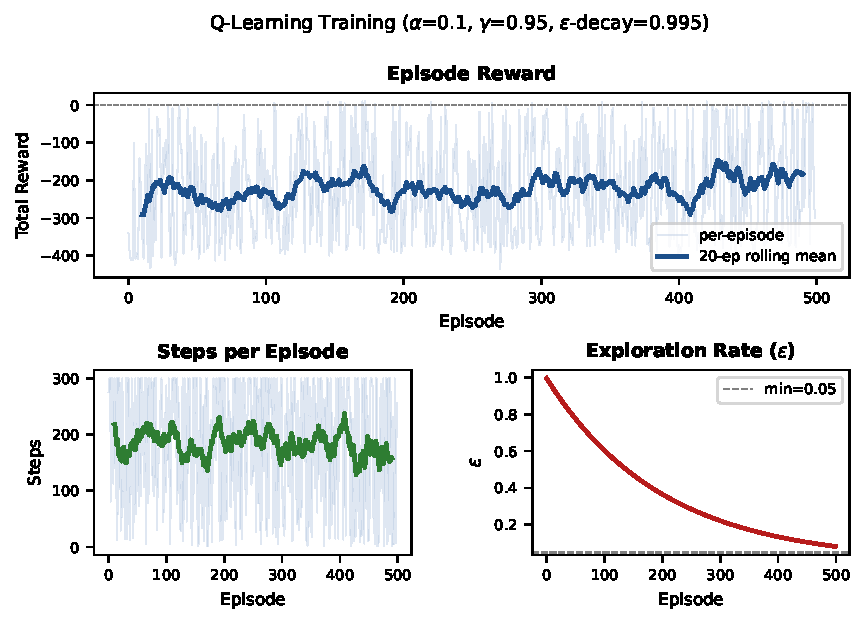
\includegraphics[width=\columnwidth]{qlearning_training.pdf}
  \caption{Representative Q-learning training curves over 500 episodes,
           generated from the trainer hyperparameters
           ($\alpha$=0.1, $\gamma$=0.95, $\varepsilon$-decay=0.995,
           max-steps=300).
           \emph{Top:} episode total reward (light) and 20-episode rolling
           mean (dark); reward increases as the policy improves.
           \emph{Bottom left:} steps per episode.
           \emph{Bottom right:} $\varepsilon$ decays from 1.0 to the
           minimum of 0.05 by episode~$\approx$500.
           Per-episode logs were not saved to disk; this curve is
           illustrative of the training dynamics under these hyperparameters.}
  \label{fig:qlearning}
\end{figure}

\subsection{OpenCV Symbol Detector}

Yongye implemented \texttt{symbol\_detector.py}, which subscribes to
\texttt{/camera/color/image\_raw} and publishes \texttt{/symbol\_detections}
as a \texttt{std\_msgs/String}:
\begin{verbatim}
label,cx,cy,confidence,area
\end{verbatim}

The detection pipeline converts each frame to grayscale, applies a 5$\times$5
Gaussian blur, performs Otsu inverse thresholding, and calls
\texttt{cv2.findContours}.
For each contour, the node computes area, perimeter, circularity
($C = 4\pi A / P^2$), polygonal vertex count, aspect ratio, and convex-hull
solidity:
\begin{itemize}
  \item $C \geq 0.80$ $\Rightarrow$ circle;
  \item vertex count $= 3$ $\Rightarrow$ triangle;
  \item vertex count $= 4$, aspect ratio $\in [0.8, 1.2]$ $\Rightarrow$ square;
  \item solidity $< 0.65$, vertex count $\geq 8$ $\Rightarrow$ star.
\end{itemize}
Contours below 800~px$^2$ are rejected as noise; very large contours are
rejected as room or wall fragments.
The detector also publishes annotated debug images on
\texttt{/symbol\_detector/debug\_image}.

\subsection{RGB-D Localizer and Symbol Map}

\texttt{symbol\_localizer.py} subscribes to \texttt{/symbol\_detections} and
the aligned depth image, samples depth at the image centroid, back-projects
the pixel into the camera frame using the intrinsics shown in
Section~\ref{sec:original-design}, and applies a TF transform to express the
result in \texttt{odom} or \texttt{map}.
\texttt{symbol\_map.py} accumulates these 3-D detections in a persistent JSON
file, keyed by label, so that detections survive node restarts.
These components are fully implemented and form the foundation for full
RGB-D symbol localization and navigation.

\subsection{Neural Network Symbol Recognition}

Nalongsone designed and built a PyTorch-based symbol recognition pipeline
as a second experiment.
The workflow involved (1)~collecting image data from the RealSense camera
at multiple viewing angles and lighting conditions; (2)~training a CNN
classifier for the four target labels; (3)~integrating the model into the
ROS pipeline using OpenCV for preprocessing; and (4)~exploring depth-image
fusion to estimate real-world 3-D positions.
A deployment path using Docker was prototyped for repeatability across
machines.
Although this approach was not used in the final demo due to hardware time
constraints, it provided a data-driven alternative to the classical contour
pipeline.

\subsection{Navigation Controller and Command Interface}

Nalongsone implemented the foundational structures for \texttt{navigation\_controller.py}
and \texttt{command\_interface.py}.
The navigation controller was designed around a proportional drive-to-pose
approach: given a target 3-D pose from the symbol map, the controller computes
the angular error and linear distance and outputs velocity commands on
\texttt{/cmd\_vel}.
The command interface provides the user-facing entry point: a request
such as ``find the triangle'' triggers a symbol-map query, which returns
the most recently observed 3-D pose, which is then passed to the navigation
controller.

\subsection{Robot Bringup and Hardware Integration}

Nalongsone led the physical robot bringup work.
This included writing \texttt{triton.launch}, configuring the TF tree
(camera frame $\to$ base link $\to$ odom), setting up RViz configurations
for LiDAR and camera visualization, enabling teleoperation over both the
Jetson desktop and SSH, and running hardware tests for SLAM and map-saving
with \texttt{gmapping}.
These integration activities were essential for validating that the sensor
drivers, TF frames, and communication topics worked correctly on the real robot
before deploying autonomous behaviors.

% -----------------------------------------------------------------------------
\section{Hardware Limitations and Engineering Adaptations}
\label{sec:adaptations}

\subsection{Q-Learning Sim-to-Real Transfer Failure}

The first significant deviation from the original plan occurred when
the Q-learning policy was deployed on the real Triton robot.
In Gazebo, the policy produced smooth exploration in the 6$\times$6~m
training room.
On the real kitchen floor, however, the same policy caused the robot to
oscillate left and right, fail to make useful forward progress, and
approach obstacles unsafely.
The root cause was a distribution mismatch between the simulated room geometry
and the real kitchen layout: the kitchen had narrow corridors, irregular
clutter (cabinets, refrigerator, trash bin), and sensor noise patterns
not present in the simulation.
States that appeared rarely in training were reached frequently in the real
environment, and the learned Q-values for those states were unreliable.

The engineering response was to replace the Q-policy with a conservative
LiDAR-based reactive explorer (\texttt{reactive\_explorer.py}).
This controller divides the RPLIDAR scan into front, left, and right sectors.
When the front sector is clear, the robot drives forward slowly.
When an obstacle is detected, the robot turns toward the side with more free
space.
A hysteresis band between the stop and clear thresholds prevents rapid
oscillation.
The controller also performs periodic in-place look-around rotations so that
the forward-mounted RealSense camera can sweep across a wider portion of the
room.
This design trades adaptability for predictability, which is the correct
trade-off when reliable hardware behavior is required for a final demo.

\subsection{RealSense USB~2.0 Bandwidth Limitation}

The second and more consequential limitation arose from the RealSense D435
camera's USB enumeration on the Jetson Nano.
The camera was expected to operate at USB~3.0 / 5000~Mbps, which is required
for stable simultaneous color and aligned-depth streaming.
On the robot, the camera instead enumerated repeatedly as USB~2.0 at 480~Mbps.
Under this bandwidth constraint, \texttt{librealsense} reported errors including
\texttt{Out of frame resources}, \texttt{USB SCP overflow}, and
\texttt{UVC stream stalled}.
The color topic (\texttt{/camera/color/image\_raw}) was sometimes inconsistent,
and the aligned depth topic
(\texttt{/camera/aligned\_depth\_to\_color/image\_raw}) was frequently unstable
or missing.

Because stable aligned depth was required for 3-D symbol localization,
this hardware issue prevented the full RGB-D pipeline from running
reliably enough to demonstrate in the final evaluation.
The engineering response was to redesign the final demo around a
USB2-compatible configuration: the RealSense was used only as a low-bandwidth
color camera, the depth localizer and symbol map were set aside for the final
demo, and the success condition was changed from ``navigate to the 3-D symbol
pose'' to ``search safely and stop when the target is reliably detected in
the 2-D color image.''

\subsection{Environment Change}

Because of the combined hardware and sensor limitations, the final demo
environment was also changed from the kitchen to a more open indoor room
(bedroom or living room).
The kitchen was a narrow, cluttered space with poor visibility for
forward-mounted cameras and many surfaces that created false contours
for the OpenCV detector.
An open room provided better ambient lighting, fewer background clutter
sources, and more floor space for the reactive explorer to navigate without
frequent obstacle encounters.
The printed symbols (pure black shapes on white A4 paper) were placed in
well-lit positions so that the color-only OpenCV pipeline could detect the
target shape reliably without depth information.

% -----------------------------------------------------------------------------
\section{Final System: USB2-Compatible Demo}
\label{sec:final-system}

\subsection{Architecture}

The final running system uses three cooperating ROS nodes, shown in
Fig.~\ref{fig:arch}.
The perception layer subscribes to the RealSense color topic and publishes
symbol detections.
The exploration layer subscribes to RPLIDAR scans and publishes velocity
commands on \texttt{/cmd\_vel}.
The target monitor subscribes to detections and disables exploration when
the requested symbol has been confirmed.

\begin{figure}[t]
\centering
\tikzset{
  hw/.style   = {rectangle, rounded corners=2pt, draw=black!70, fill=gray!15,
                 minimum width=1.4cm, minimum height=0.46cm,
                 font=\tiny\ttfamily, align=center, inner sep=2pt},
  rosnode/.style={rectangle, rounded corners=2pt, draw=black!80, fill=blue!14,
                 minimum width=1.55cm, minimum height=0.46cm,
                 font=\tiny\ttfamily\bfseries, align=center, inner sep=2pt},
  topic/.style= {ellipse, draw=black!55, fill=orange!20,
                 minimum width=1.55cm, minimum height=0.40cm,
                 font=\tiny\ttfamily, align=center, inner sep=1pt},
  arr/.style  = {-{Stealth[length=3pt]}, semithick, black!65},
  lbl/.style  = {font=\tiny, fill=white, inner sep=1pt},
}
\scalebox{0.82}{%
\begin{tikzpicture}[node distance=0.38cm and 0.52cm]

%% ── Row 1: camera pipeline ──────────────────────────────────────────────────
\node[hw]                          (cam)  {RealSense\\(color only)};
\node[topic,   right=of cam]       (img)  {/camera/color\\image\_raw};
\node[rosnode, right=of img]       (det)  {symbol\_\\detector.py};
\node[topic,   right=of det]       (sdp)  {/symbol\_\\detections};

%% ── Row 2: LiDAR pipeline ───────────────────────────────────────────────────
\node[hw,      below=0.80cm of cam] (lid)  {RPLIDAR};
\node[topic,   right=of lid]        (scn)  {/scan};
\node[rosnode, right=of scn]        (exp)  {reactive\_\\explorer.py};
\node[topic,   right=of exp]        (cmd)  {/cmd\_vel};

%% ── Stop monitor (centred vertically, to the right of /symbol_detections) ───
\node[rosnode, below=0.38cm of sdp] (mon)  {stop\_\\monitor.py};

%% ── /exploration_enabled output ─────────────────────────────────────────────
\node[topic, below=0.38cm of mon]   (enb)  {/exploration\\\_enabled};

%% ── Arrows ───────────────────────────────────────────────────────────────────
\draw[arr] (cam) -- (img);
\draw[arr] (img) -- (det);
\draw[arr] (det) -- (sdp);
\draw[arr] (lid) -- (scn);
\draw[arr] (scn) -- (exp);
\draw[arr] (exp) -- (cmd);
\draw[arr] (sdp) -- (mon);
\draw[arr] (mon) -- (enb);
% feedback: /exploration_enabled → explorer (dashed)
\draw[arr, dashed, gray!70]
      (enb.west) -- ++(-0.35,0) |- node[lbl,pos=0.75]{stop} (exp.south);

%% ── Background group labels ──────────────────────────────────────────────────
\begin{scope}[on background layer]
  \node[draw=gray!40,   fill=gray!5,   rounded corners=3pt, dashed,
        fit=(cam)(lid), inner sep=4pt,
        label={[font=\tiny\itshape,gray!70]left:Hardware}] {};
  \node[draw=blue!30,   fill=blue!4,   rounded corners=3pt, dashed,
        fit=(det)(exp)(mon), inner sep=4pt,
        label={[font=\tiny\itshape,blue!60!black]above:ROS Nodes}] {};
  \node[draw=orange!45, fill=orange!3, rounded corners=3pt, dashed,
        fit=(img)(scn)(sdp)(cmd)(enb), inner sep=4pt,
        label={[font=\tiny\itshape,orange!70!black]above:Topics}] {};
\end{scope}

\end{tikzpicture}}% end scalebox
  \caption{Final USB2-compatible demo architecture. Hardware sources (gray)
           feed ROS topics (orange) consumed by three nodes (blue).
           The stop monitor latches \texttt{/exploration\_enabled=false}
           (dashed) to halt the explorer after repeated high-confidence
           detections.}
  \label{fig:arch}
\end{figure}

\subsection{Target Stop Monitor}

\texttt{star\_stop\_monitor.py} (generalized for any target label) subscribes
to \texttt{/symbol\_detections} and maintains a rolling window of recent
accepted target detections.
The final commit parameters were:
\begin{verbatim}
target_label    = triangle
min_confidence  = 0.80
commit_k        = 3
commit_window_s = 2.0
border_reject   = 30 px
\end{verbatim}

The border rejection rule (30~px from any image edge) was added after an
early false positive: a dark shadow or wall corner near the left edge of
the image was classified as a triangle with \texttt{cx = 6--8} and
confidence $\approx 0.58$--$0.67$.
Raising the threshold to 0.80 and rejecting border detections eliminated
this spurious stop while keeping sensitivity to genuine high-contrast targets.

On commit, the monitor latches \texttt{/exploration\_enabled = false},
which causes the reactive explorer to publish zero velocity and stop the robot.
The monitor also writes a JSON result file recording the reason, elapsed time,
detection counts, and any available pose.

% -----------------------------------------------------------------------------
\section{Experiments}
\label{sec:experiments}

\subsection{Experimental Setup}

The final deliverable required code, a demonstration video, and this report.
The physical experiment was run on the Triton robot in a furnished indoor room.
The robot was operated headlessly over SSH.
The target symbol (triangle) was printed on white A4 paper and placed in
the room at a location unknown to the robot at launch.
All navigation used RPLIDAR reactive control; all perception used the
low-bandwidth RealSense color stream.

\subsection{False Positive Debugging}

During early trials, the confidence threshold was set to $c_{\min} \approx 0.55$.
At that setting the system stopped on a false triangle detection at the far
left image edge (\texttt{cx = 6--8}, confidence $\approx 0.58$--$0.67$).
The source was likely a dark line, shadow, or wall corner approximated as a
triangle by the contour polygon.
Three protections were introduced: (1)~raise $c_{\min}$ to 0.80;
(2)~reject target detections within 30~px of the image boundary;
(3)~log every accepted detection with label, centroid, confidence, area,
and save a debug snapshot at commit time.
These changes made the stop decision depend on repeated, spatially central,
high-confidence contours, rather than a single weak edge artifact.

\subsection{Final Triangle Search Result}

Table~\ref{tab:params} shows the final monitor parameters, and
Table~\ref{tab:result} summarizes the result of the successful run.

\begin{table}[h]
\centering
\caption{Final target-monitor parameters.}
\label{tab:params}
\begin{tabular}{lr}
\toprule
Parameter & Value \\
\midrule
Target label & triangle \\
Minimum confidence & 0.80 \\
Commit count $K$ & 3 \\
Commit window $W$ & 2.0~s \\
Image-edge rejection & 30~px \\
\bottomrule
\end{tabular}
\end{table}

\begin{table}[h]
\centering
\caption{Final real-robot demo result.}
\label{tab:result}
\begin{tabular}{lr}
\toprule
Field & Value \\
\midrule
Reason & found\_target \\
Commit time & 151.78~s \\
Elapsed time & 161.878~s \\
Target detections & 4 \\
Total detections & 53 \\
Commit confidences & 0.990, 0.991, 0.991 \\
Pose & null (color-only) \\
\bottomrule
\end{tabular}
\end{table}

The robot explored the room for approximately 2.5 minutes before the camera
came into view of the triangle.
The three commit detections had confidence approximately 0.990--0.991, all
well above the 0.80 threshold and free from image-edge proximity.
The monitor published \texttt{/exploration\_enabled = false}, and the
explorer stopped the robot.
The null pose is expected: since the final demo intentionally disabled depth
streaming, no 3-D symbol pose was computed.

\subsection{Discussion: What the Demo Proves and What It Does Not}

The final demo proves that the full autonomous search loop works on real
hardware under the available sensor constraints.
The robot moves safely using LiDAR reactive control, processes live color
images, detects the requested triangle with OpenCV, and stops reliably after
repeated high-confidence detections.

The final demo does not prove that the depth-backprojection localizer
produces a valid 3-D symbol pose, that the symbol is inserted into the
persistent map, or that the robot drives to a measured distance threshold
from the symbol.
Those components are implemented in the codebase (localizer, map, navigation
controller) and were designed for the full pipeline, but their validation
requires a reliable USB~3.0 RealSense connection that was not available on
the robot during final integration.

The distinction matters because it separates what was \emph{built} from what
was \emph{validated on hardware}.
All subsystems were implemented; only the final, narrower behavior was
confirmed in the live demo.

\subsection{Limitations}

\textbf{Q-learning sim-to-real gap.}
The Q-policy was trained in a bounded, simplified Gazebo room.
The real environment had different geometry, dynamic clutter, and sensor
noise not represented in simulation.
Better transfer would require domain randomization, a more representative
training world, or online fine-tuning on the physical robot.

\textbf{RealSense USB bandwidth.}
The D435 did not enumerate at USB~3.0 speed on the Jetson Nano during final
integration, making stable aligned RGB-D streaming unavailable.
This is the primary reason the final demo does not include 3-D localization.

\textbf{Camera field of view.}
The RealSense is forward-mounted and low on the robot.
Symbols mounted high or to the side of the robot's path may be missed without
deliberate look-around behavior.

\textbf{Classical vision sensitivity.}
The OpenCV contour detector works well for high-contrast printed symbols
on clean backgrounds but is susceptible to shadows, dark edges, and clutter
at low confidence thresholds.
A learned detector (such as the neural-network prototype) would be more
robust in varied conditions.

% -----------------------------------------------------------------------------
\section{Additional Experiment}
\label{sec:additional-experiment}

In addition to the group pipeline described above, we performed an additional
experiment focused on replacing hand-designed shape rules with a trained
neural-network classifier and deploying that classifier inside the real-robot
ROS package \texttt{symbols\_recognition}.
This experiment followed the practical workflow shown in
Fig.~\ref{fig:add-workflow}: collect RGB symbol images, train a classifier,
load the checkpoint in ROS, publish live predictions, and use the prediction
stream to command the Triton robot toward a requested symbol. The result record video for this experiment is available at
\\ \url{https://www.youtube.com/watch?v=vd26c0NDQ-E}; \\ it documents the real
project workflow and demonstration, including camera-based symbol observation,
trained-model recognition, ROS integration, and the connection between
perception output and Triton robot behavior.

\begin{figure}[t]
  \centering
  \tikzset{
    addstep/.style={rectangle, rounded corners=2pt, draw=black!70,
                    fill=blue!10, minimum width=1.55cm,
                    minimum height=0.48cm, font=\tiny\bfseries,
                    align=center, inner sep=2pt},
    addarr/.style={-{Stealth[length=3pt]}, semithick, black!65}
  }
  \scalebox{0.86}{%
  \begin{tikzpicture}[node distance=0.38cm and 0.33cm]
    \node[addstep] (collect) {Collect\\RGB images};
    \node[addstep, right=of collect] (train) {Train\\classifier};
    \node[addstep, right=of train] (load) {Load ROS\\checkpoint};
    \node[addstep, below=of load] (predict) {Publish live\\predictions};
    \node[addstep, left=of predict] (command) {Command\\Triton};
    \node[addstep, left=of command] (demo) {Record\\demo};
    \draw[addarr] (collect) -- (train);
    \draw[addarr] (train) -- (load);
    \draw[addarr] (load) -- (predict);
    \draw[addarr] (predict) -- (command);
    \draw[addarr] (command) -- (demo);
  \end{tikzpicture}}%
  \caption{Additional experiment workflow: camera-based data collection,
           neural-network training, ROS inference, and planned use of depth
           and navigation for symbol-directed robot behavior.}
  \label{fig:add-workflow}
\end{figure}

\subsection{Experimental Setup}

The dataset was collected from RealSense RGB video of printed black symbols
on white paper in an indoor room.
The raw frames were sorted into four class folders:
\texttt{circles}, \texttt{squares}, \texttt{stars}, and \texttt{triangles}.
The final dataset contained 3099 training images, 504 validation images, and
530 test images.
Figure~\ref{fig:add-dataset} shows representative training images copied from
the actual dataset.

\begin{figure}[t]
  \centering
  \begin{minipage}{0.235\columnwidth}
    \centering
    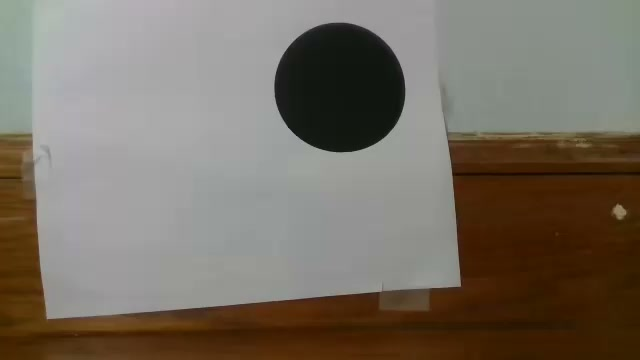
\includegraphics[width=\linewidth]{additional_circle_sample.jpg}\\
    \scriptsize circle
  \end{minipage}
  \begin{minipage}{0.235\columnwidth}
    \centering
    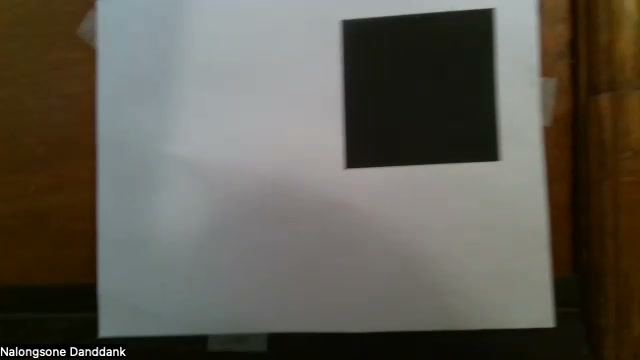
\includegraphics[width=\linewidth]{additional_square_sample.jpg}\\
    \scriptsize square
  \end{minipage}
  \begin{minipage}{0.235\columnwidth}
    \centering
    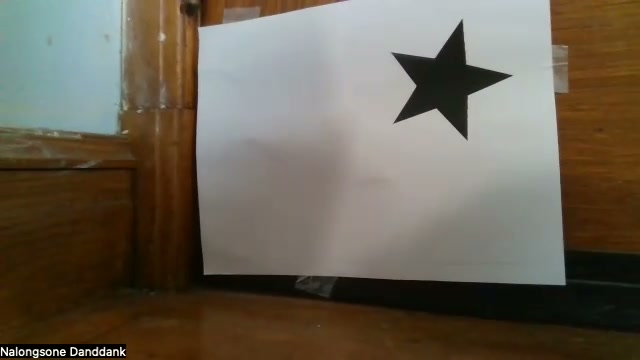
\includegraphics[width=\linewidth]{additional_star_sample.jpg}\\
    \scriptsize star
  \end{minipage}
  \begin{minipage}{0.235\columnwidth}
    \centering
    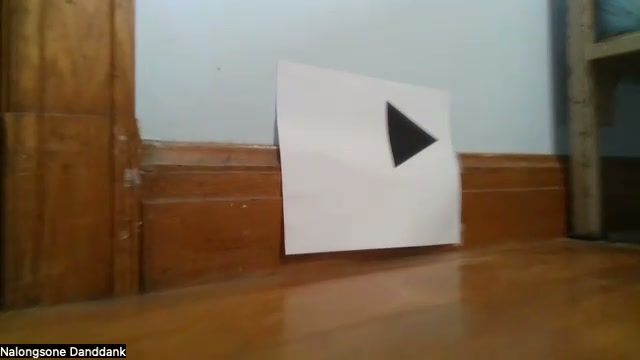
\includegraphics[width=\linewidth]{additional_triangle_sample.jpg}\\
    \scriptsize triangle
  \end{minipage}
  \caption{Representative training images used for the neural-network
           symbol-recognition experiment.}
  \label{fig:add-dataset}
\end{figure}

Two PyTorch classifiers were trained in the \texttt{nn\_training} folder.
The first was a custom CNN with 128$\times$128 input images, batch size 64,
AdamW optimization, class weighting, and a maximum of 40 epochs.
The second was a MobileNetV2 classifier with 224$\times$224 input images,
batch size 32, AdamW optimization, and 40 epochs.
Both training scripts saved the best and latest checkpoints, a
\texttt{history.csv} file, dataset counts, test metrics, and a plotted result
summary.
The trained checkpoints used by ROS were:
\path{cnn/checkpoints/symbols_cnn_best.pt} and
\path{mobilenetv2/checkpoints/symbols_mobilenetv2_best.pt}.

For deployment, the project used an Ubuntu~20.04 Docker image with ROS Noetic,
\texttt{cv\_bridge}, OpenCV, \texttt{usb\_cam}, RPLIDAR support, PyTorch, and
the catkin workspace.
The Docker Compose service used host networking and mounted
\texttt{nn\_training} read-only at \texttt{/nn\_training}, which made the
trained checkpoints available to the ROS classifier node.
The runtime entry point was:
\begin{verbatim}
docker compose exec \
  triton_noetic_ping \
  /setup.bash \
  target_symbol:=triangle
\end{verbatim}
or, inside the container:
\begin{verbatim}
roslaunch symbols_recognition \
  real_robot.launch \
  target_symbol:=triangle
\end{verbatim}

\subsection{Software and Hardware Debugging}

Most debugging time was spent on the boundary between working Python models
and reliable robot execution.
On the software side, the Docker container had to be configured with
\texttt{network\_mode: host}, the correct \texttt{ROS\_MASTER\_URI} and
\texttt{ROS\_IP}, and direct access to \texttt{/dev} so that ROS sensor
drivers could see the camera and LiDAR.
Because the catkin source tree was mounted into the container, the workspace
also had to be rebuilt with \texttt{catkin build} after source-code changes.

The classifier node introduced a second class of errors.
If \texttt{/symbol\_classifier/result} appeared in \texttt{rostopic list} but
\texttt{rosnode list} did not show \texttt{/symbol\_classifier}, the topic was
only present because another node subscribed to it; the classifier process had
actually exited.
Running
\begin{verbatim}
rosrun symbols_recognition \
  symbol_classifier.py \
  _checkpoint_path:=/nn_training/cnn/\
    checkpoints/symbols_cnn_best.pt \
  _image_topic:=/camera/color/image_raw
\end{verbatim}
was the most useful diagnostic because it exposed missing-checkpoint, PyTorch,
and image-topic errors directly in the terminal.
The launch file was also used to pass an explicit checkpoint path, avoiding
ambiguity between CNN and MobileNetV2 checkpoints.

The largest hardware issue was camera reliability.
The original plan assumed the RealSense D435 would provide stable RGB-D data,
but on the robot it often behaved as a low-bandwidth or incorrectly selected
USB video source.
Observed symptoms included RealSense driver failures, missing camera topics,
green or purple web-video streams, warped images, and incorrect
\texttt{/dev/video*} endpoints.
The practical workaround was to run the final additional experiment with
\texttt{usb\_cam}, select the RGB endpoint manually, and verify the pixel
format with:
\begin{verbatim}
v4l2-ctl --list-devices
v4l2-ctl --list-formats-ext \
  -d /dev/video2
\end{verbatim}
For the real robot, \texttt{/dev/video2} with \texttt{yuyv} was the most useful
default, but the index could change between boots.

\subsection{Search and Recognition Symbols}

The trained models performed very well on the held-out data from the same
collection process.
The custom CNN reached 100.0\% test accuracy on 530 test images, while
MobileNetV2 reached 99.81\% test accuracy.
Figures~\ref{fig:add-cnn-results} and \ref{fig:add-mobilenet-results} show
the saved training curves and summary plots generated by the project scripts.

\begin{figure}[t]
  \centering
  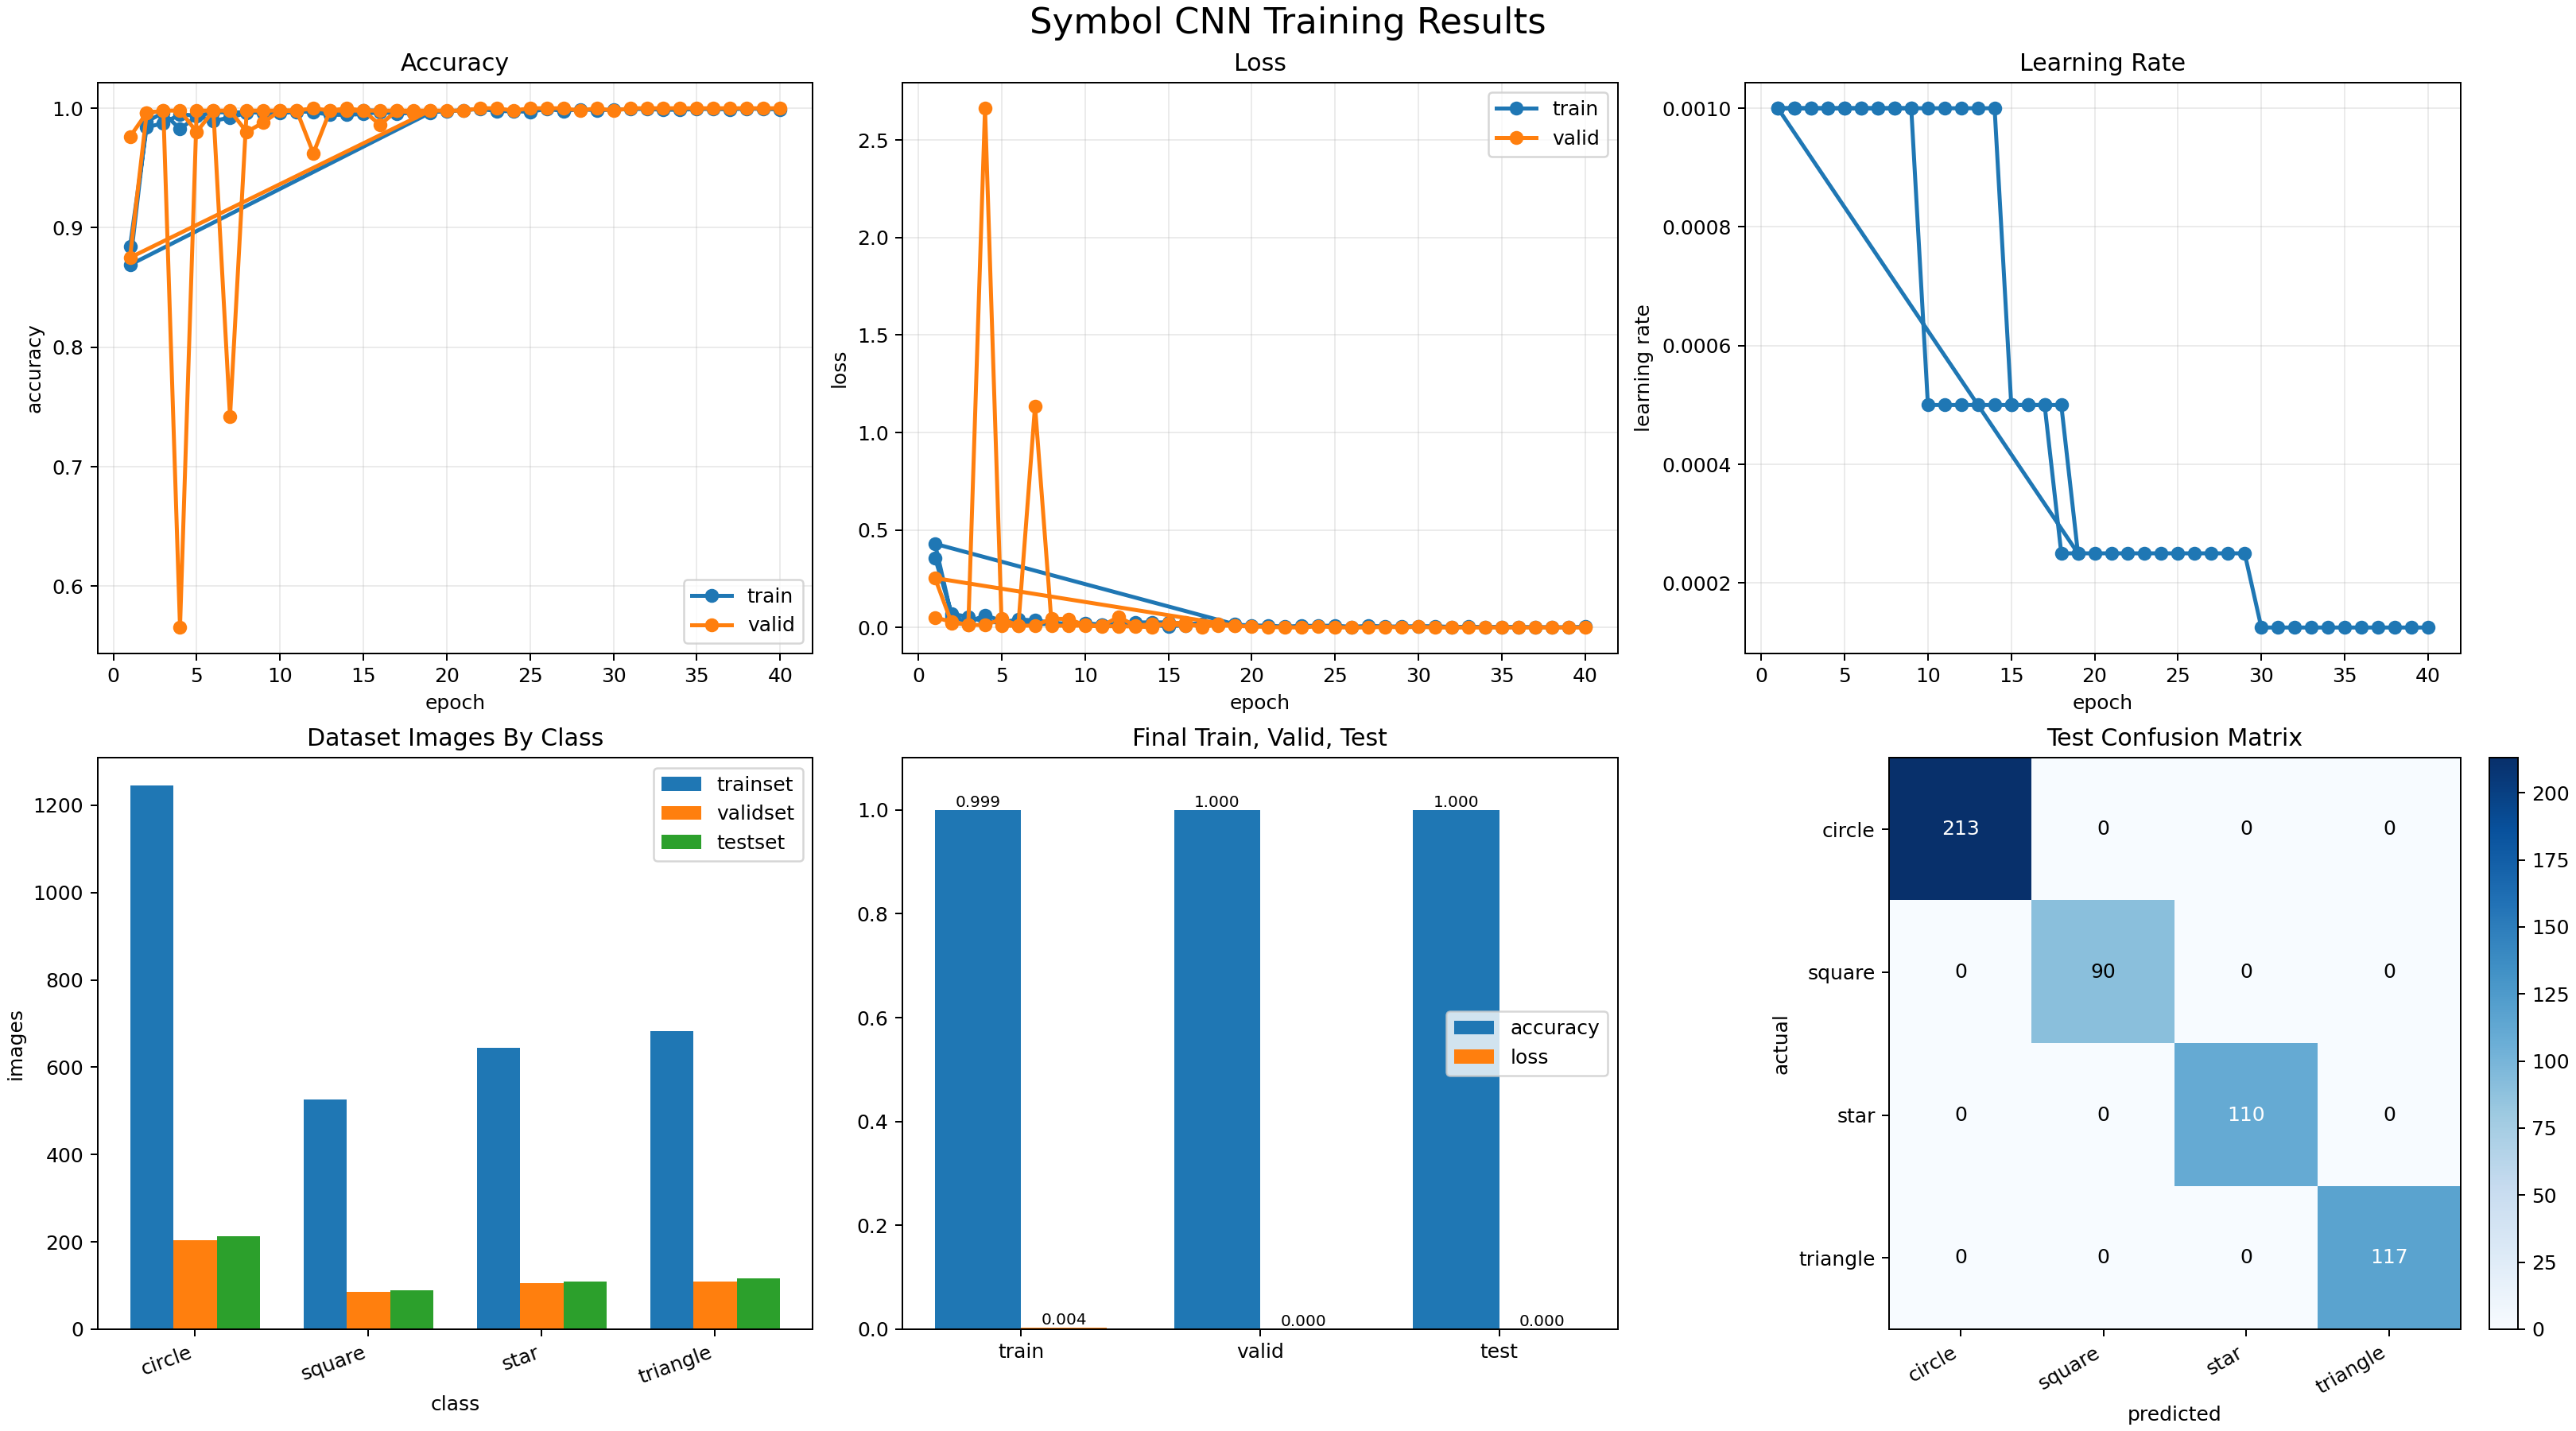
\includegraphics[width=\columnwidth]{additional_cnn_results.png}
  \caption{Saved CNN training summary, including train/validation accuracy,
           loss, learning rate, dataset counts, final metrics, and confusion
           matrix.}
  \label{fig:add-cnn-results}
\end{figure}

\begin{figure}[t]
  \centering
  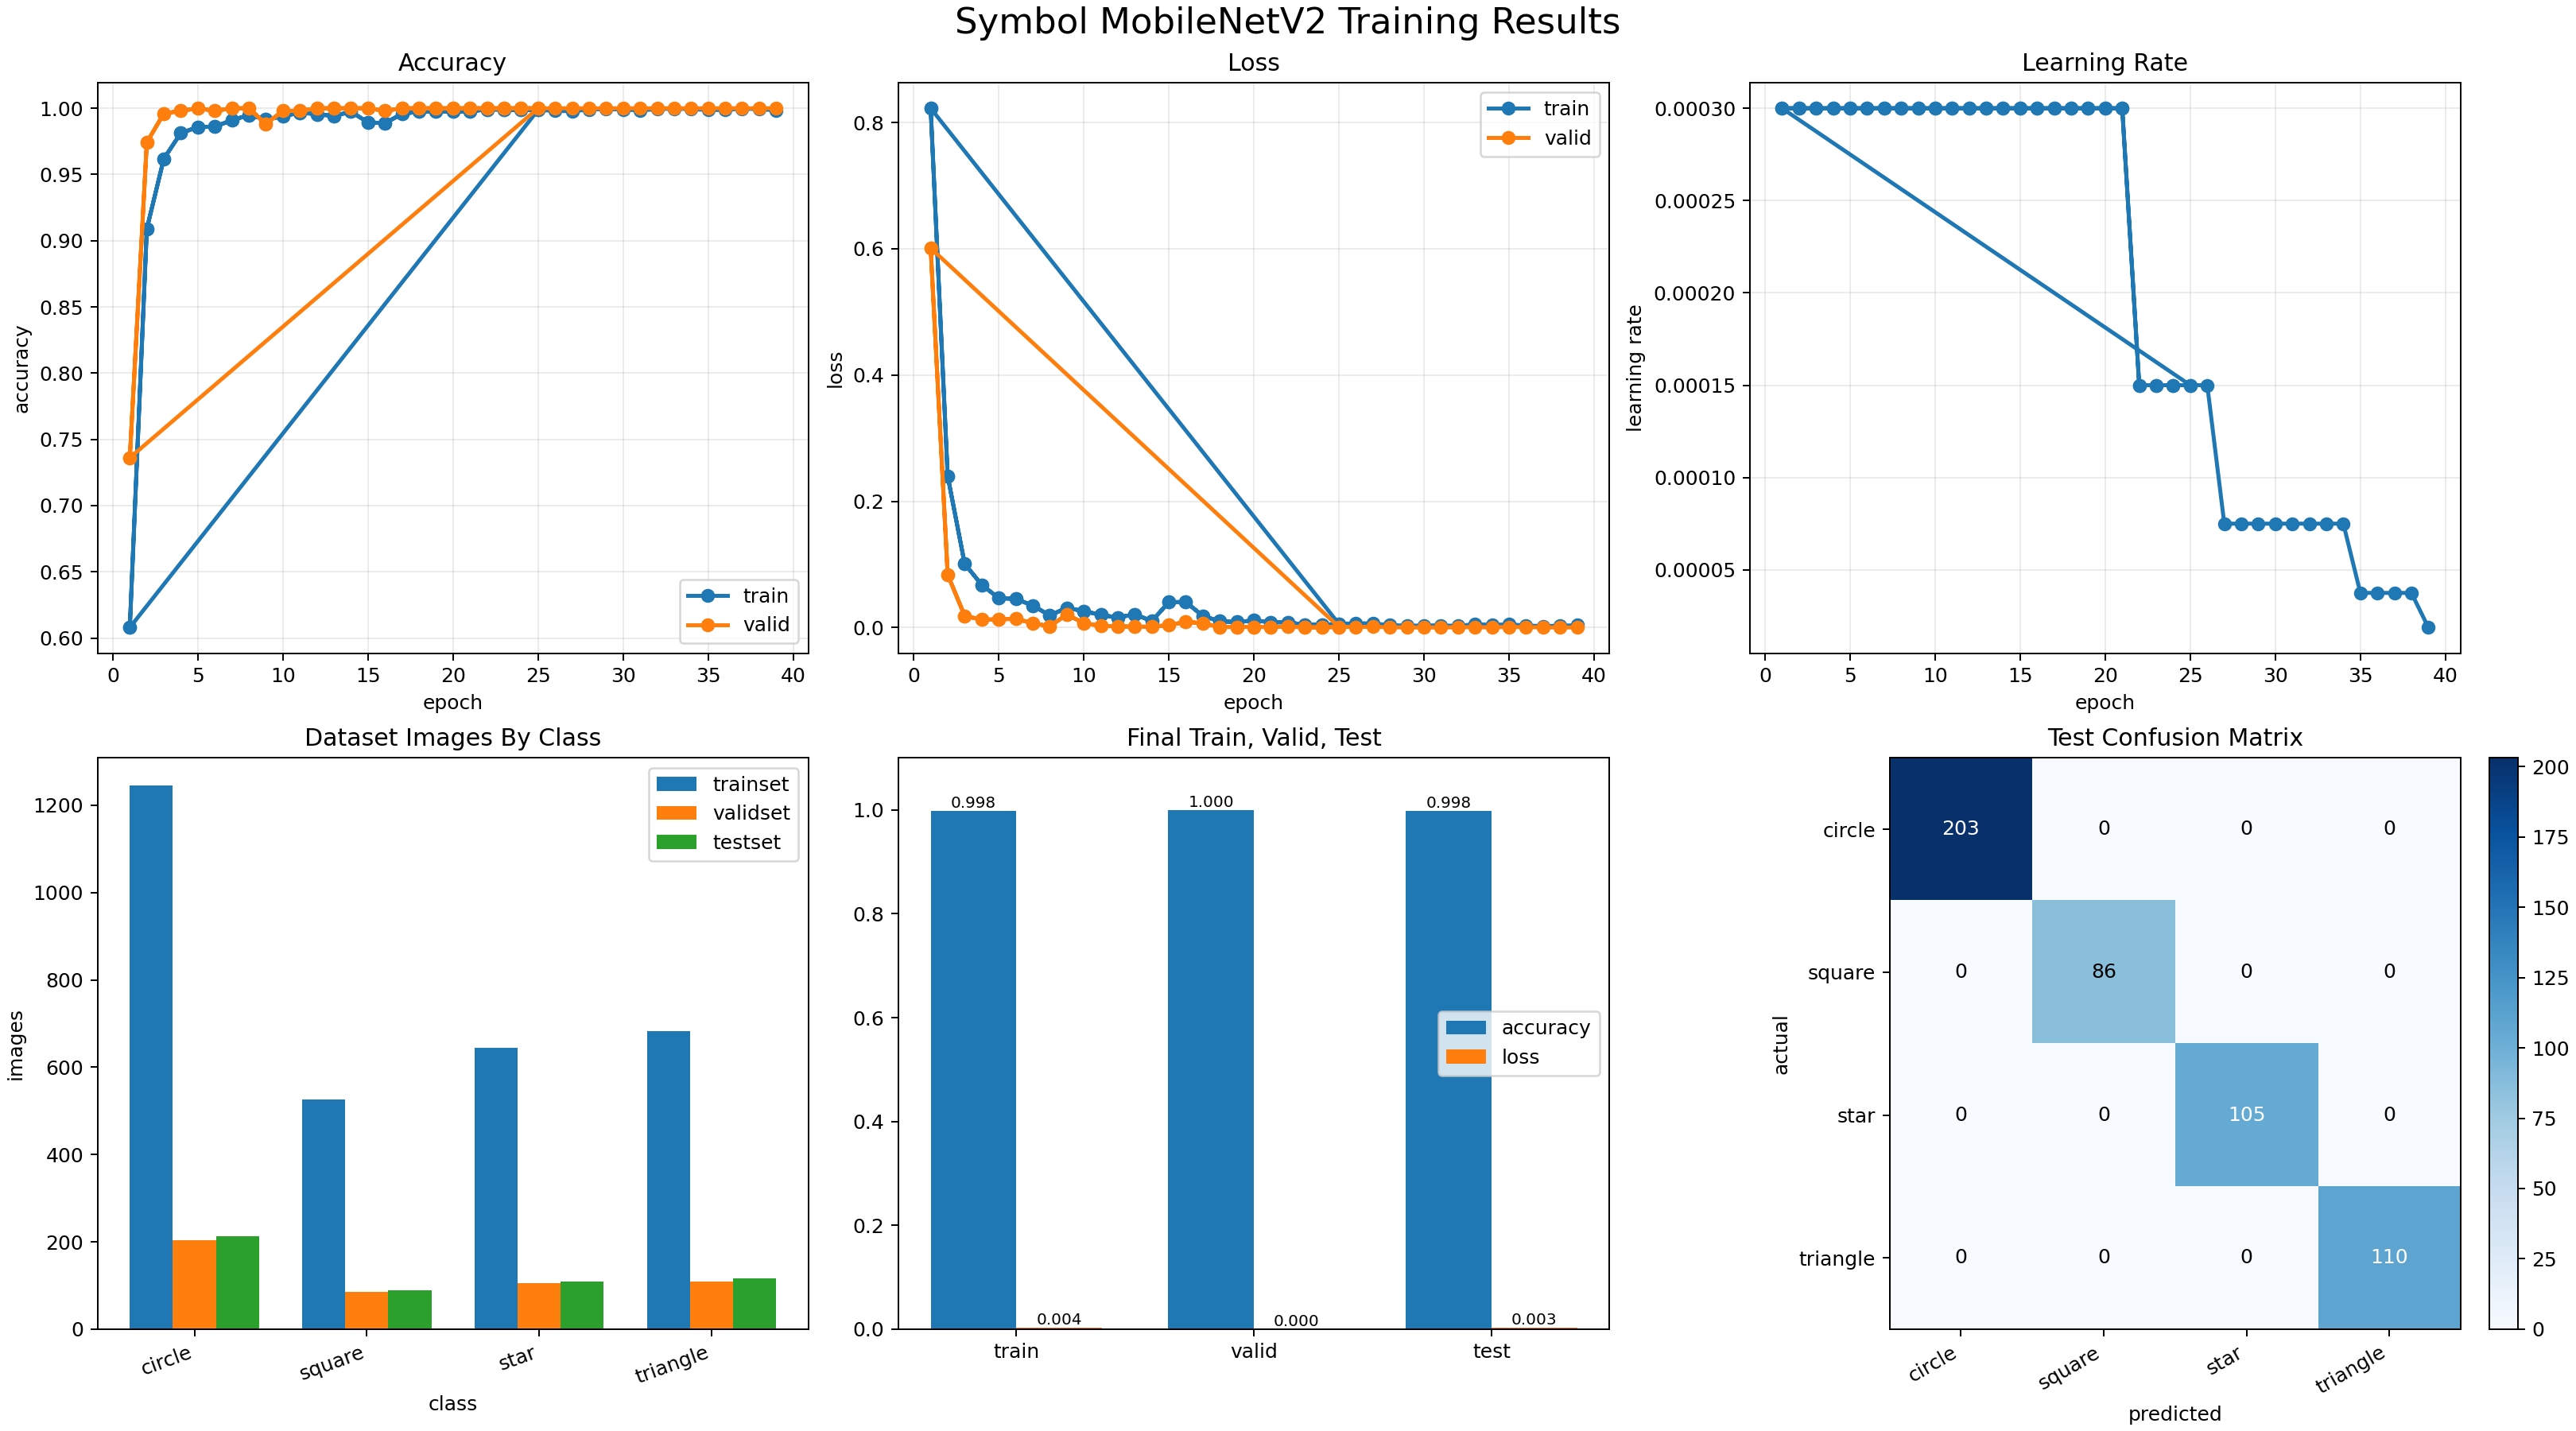
\includegraphics[width=\columnwidth]{additional_mobilenetv2_results.png}
  \caption{Saved MobileNetV2 training summary for the same four-symbol
           dataset.}
  \label{fig:add-mobilenet-results}
\end{figure}

\begin{table}[t]
\centering
\caption{Additional neural-network dataset and test results.}
\label{tab:add-nn-results}
\renewcommand{\arraystretch}{1.08}
\begin{tabular}{lrr}
\toprule
Item & CNN & MobileNetV2 \\
\midrule
Input size & 128$\times$128 & 224$\times$224 \\
Training images & 3099 & 3099 \\
Validation images & 504 & 504 \\
Test images & 530 & 530 \\
Test accuracy & 1.0000 & 0.9981 \\
Test loss & $2.91{\times}10^{-5}$ & 0.00295 \\
\bottomrule
\end{tabular}
\end{table}

In ROS, \texttt{symbol\_classifier.py} loads the checkpoint, subscribes to
\texttt{/camera/color/image\_raw}, and publishes the predicted label,
confidence, full JSON result, and optional annotated image.
The controller \texttt{target\_symbol\_controller.py} subscribes to the JSON
result and \texttt{/scan}.
Its behavior is: rotate while searching, align the target toward the image
center, move forward while the target remains visible, and stop when the front
LiDAR range falls below \texttt{stop\_distance}.

The experiment was successful for the perception portion: the trained model
could classify the four printed symbols and publish usable ROS results.
The robot-level search behavior was partially successful.
The robot could be launched with a target such as \texttt{triangle}, receive
classifier output, and connect that output to velocity decisions.
However, full autonomous ``search, recognize, localize in 3-D, and navigate to
the symbol'' was not fully validated because the depth stream and RealSense
hardware path were not reliable enough for the RGB-D part of the proposal.

\subsection{Discussion}

The beginning proposal was more ambitious than the final real-robot result.
The intended system was an end-to-end semantic navigation stack: collect RGB-D
data, train a neural-network classifier, run the classifier in ROS, use depth
to recover the real-world 3-D position of each symbol, store those positions,
and navigate to a user-requested target.
The additional experiment achieved the data collection, training, model
checkpointing, Docker deployment, ROS classifier node, and target-controller
integration pieces.
It also demonstrated that the symbol classes are learnable with a compact CNN
and MobileNetV2 under the collected-data conditions.

The final reality was narrower.
Because the RealSense and USB camera path was unstable, the most reliable
robot behavior used RGB-only recognition with LiDAR-based stopping rather than
complete RGB-D localization and semantic map navigation.
This is still a useful robotics result: it converted an image classifier into
a live ROS perception stream and connected that stream to robot motion.
The experiment also clarified which parts of the original proposal were
algorithmically solved and which parts remained blocked by hardware and
integration constraints.

\subsection{Limitations}

The main dataset limitation is that the images came from a small number of
recorded indoor scenes with the same printed symbol style.
Although the test accuracy is high, the train, validation, and test frames are
from the same visual domain, so the reported accuracy is likely optimistic for
new rooms, different lighting, different paper sizes, motion blur, or cluttered
backgrounds.
The dataset is also imbalanced: the training split contains 1246 circle images
but only 527 square images.
Class weighting helped training, but it does not replace broader data
collection.
Another limitation is that the classifier has only four symbol classes; unless
a background or ``none'' class is added, the network is forced to choose one of
the four symbols even when the camera sees no valid target.

The model limitation is therefore not only numerical accuracy.
CNN test accuracy of 100.0\% and MobileNetV2 test accuracy of 99.81\% show that
the saved models fit this dataset, but they do not prove open-world robustness.
For a stronger experiment, the test set should be collected in a separate room,
under different lighting, with negative/background images, partial occlusions,
and symbols at different distances.

The integration limitation is the hardest one.
The ROS package can load the checkpoint and publish symbol predictions, but the
real robot still depends on correct camera enumeration, USB bandwidth, ROS
network variables, catkin workspace state, and checkpoint paths.
The RealSense camera did not consistently provide the expected RGB-D stream,
so the depth-image part of the original proposal could not be relied on.
Consequently, the additional experiment validated 2-D recognition and partial
target-directed motion, but not the full 3-D symbol mapping and
navigation-to-symbol behavior originally proposed.

% -----------------------------------------------------------------------------
\section{Conclusion}
\label{sec:conclusion}

This project designed, implemented, and tested an autonomous symbol-search
stack for the physical Triton robot.
The original goal---Q-learning exploration, RGB-D detection, 3-D symbol
localization, persistent symbol mapping, and navigation-to-symbol---guided
the system architecture and was implemented as a codebase.
The final group demonstration validated a narrower but real behavior:
the robot explored safely, processed live sensor data, recognized the
requested triangle in the color stream, and stopped after repeated
high-confidence detections.

The additional experiment extended this work with a data-driven recognition
pipeline.
RealSense RGB frames were organized into a four-class dataset, two PyTorch
models were trained, and the resulting checkpoints were integrated into the
\texttt{symbols\_recognition} ROS package through Docker and ROS launch files.
The CNN reached 100.0\% test accuracy and MobileNetV2 reached 99.81\% on the
held-out dataset, showing that the collected symbols were learnable by neural
models.
The ROS integration also showed how trained model output can be converted
into live topics for target-directed robot behavior.

The gap between the proposal and the final result came mainly from physical
deployment constraints.
The Q-learning policy trained in Gazebo did not transfer reliably to the real
environment, so the final system used a conservative LiDAR reactive explorer.
The RealSense camera did not consistently provide the expected stable RGB-D
stream on the Triton hardware, so full depth-based 3-D localization, persistent
symbol mapping, and navigation to a measured symbol pose were not fully
validated.
These constraints reduced the final behavior, but they also clarified which
parts of the pipeline were algorithmically complete and which parts remained
hardware-limited.

Future work should connect the strongest parts of both experiments.
Restoring a stable USB~3.0 RealSense RGB-D stream would enable 3-D symbol
localization and semantic mapping.
Collecting a broader dataset with background images, new rooms, varied
lighting, blur, and partial occlusion would make the neural classifier more
robust outside the recorded training domain.
Replacing the contour detector with the trained classifier in the final
real-robot loop would reduce false positives, and improving the simulation
with domain randomization would make learned exploration more transferable.
Finally, combining SLAM, the symbol map, and the navigation controller would
complete the original semantic landmark architecture: search, recognize,
remember, and navigate to a user-requested symbol.

% -----------------------------------------------------------------------------
\appendix
\section*{Appendix: Workload Report}

The workload distribution below covers the full group project, including
proposal planning, robot bringup, simulation, perception, exploration,
integration, demonstrations, and report preparation.
The percentages reflect actual contributions and are agreed upon by all
team members.

\begin{table}[h]
\centering
\caption{Full-project workload distribution.}
\label{tab:workload}
\renewcommand{\arraystretch}{1.18}
\begin{tabular}{@{}p{1.7cm} p{5.1cm} c@{}}
\toprule
\textbf{Member} & \textbf{Responsibilities and contributions} & \textbf{\%} \\
\midrule
Chengtao Lin
  & Designed the Gazebo simulation setup and Q-learning formulation;
    implemented shared RL utilities (\texttt{rl\_common.py}),
    state discretization, Q-table training
    (\texttt{q\_learning\_trainer.py}), and exploration-controller code
    (\texttt{exploration\_controller.py});
    generated Gazebo symbol textures and world files;
    evaluated why the learned policy did not transfer to the real kitchen
    and supported the switch to reactive exploration;
    supported robot SLAM experiments, demo recording, result
    interpretation, and final paper writing.
  & 34 \\[2pt]
Yongye Tan
  & Implemented the OpenCV symbol-detection pipeline
    (\texttt{symbol\_detector.py}), including contour features, confidence
    scoring, debug snapshots, and false-positive hardening;
    developed the depth-localization node (\texttt{symbol\_localizer.py})
    and persistent symbol-map prototype (\texttt{symbol\_map.py});
    implemented and tuned the reactive explorer
    (\texttt{reactive\_explorer.py}) and target stop monitor
    (\texttt{star\_stop\_monitor.py});
    ran hardware experiments, collected final demo metrics, and contributed
    to report results, experiments, and discussion sections.
  & 33 \\[2pt]
Nalongsone Danddank
  & Led ROS bringup and hardware integration for the physical Triton,
    including \texttt{triton.launch}, TF wiring, RViz configuration,
    teleoperation, and launch-file integration;
    implemented the navigation-controller prototype
    (\texttt{navigation\_controller.py}) and command interface
    (\texttt{command\_interface.py});
    led the additional experiment by collecting multi-angle image data,
    training CNN and MobileNetV2 symbol classifiers, plotting training
    results, and integrating checkpoints into the Docker/ROS
    \texttt{symbols\_recognition} pipeline;
    helped with hardware testing, system integration, demo preparation,
    and presentation and report materials.
  & 33 \\
\midrule
\textbf{Total} & & \textbf{100} \\
\bottomrule
\end{tabular}
\end{table}

\end{document}
